\documentclass[a4paper]{jpconf}
\usepackage{graphicx}
\begin{document}
\title{Upgrades to the SINQ Cold Neutron Source}

\author{R M Bergmann, U Filges, D Kiselev, T Reiss, V Talanov and M Wohlmuther}

\address{Paul Scherrer Institut, 5232 Villigen, Switzerland}

\ead{ryan.bergmann@psi.ch}

\begin{abstract}Changing the configuration of the cold neutron source during an extended shutdown of Swiss Spallation Neutron Source (SINQ) is being considered for improving performance of the instruments that use the cold source.  The cold neutron source consists of a 20 L volume of liquid D$_2$ at approximately 25 K.  Previous upgrades included adding a re-entrant hole into one side of the D$_2$ volume to allow cold neutrons to stream uninhibited from the center of the source towards the instrument neutron guides.  Calculations done prior to these changes predicted cold neutron fluence gains from 1.2 to 1.6, with gains increasing with wavelength. These increases have not been observed, and it is suspected that the re-entrant hole is not fully voided.  Voiding the re-entrant hole relies on radiative heating to boil D$_2$ which in turn fills the re-entrant hole cavity, pushing the liquid D$_2$ out.  Proposed plans include making the re-entrant hole external (ensuring that it is not filled with liquid D$_2$), removing some extra structural material around the D2 tank, redesigning the re-entrant hole geometry to be more optically ideal, introducing a Pb-208 reflector to minimize cold neutron up-scattering from the surrounding D$_2$O moderator tank, and implementing a small liquid H$_2$ volume to provide a cold neutron “hot spot” for certain instruments.  These changes are predicted to increase neutron fluence between 1.1 to 2.0 times the current levels, depending on instrument location, view, and wavelengths of interest.
\end{abstract}

\ack{This work was supported by Swiss National Science Foundation grant 200021\_150048/1.}

\section{Introduction}

There is a planned shutdown of the Swiss Spallation Neutron Source (SINQ) in 2017, which provides an opportunity for changes to be made to the liquid deuterium cold neutron source.  The 20 liter volume of liquid D$_2$ at approximately 25 K is located within the D$_2$O moderator tank surrounding the Pb spallation target.  The innermost face of the cold source is approximately 35 cm away from the center of the target.  In the planned upgrade strategies, no changes to the surrounding aluminium and zirconium safety hulls will be made, and no changes to the insert tube structure will be made.  I.e., all changes must fit into the existing multi-walled insert geometry.  

\section{Re-entrant Hole}

The goal of the re-entrant hole (REH) is to remove scattering and absorbing material between the cold neutron maximum and the direction of interest.  In this case, the cold neutron maximum is at the center of the cold source and the direciton of interest is towards the SINQ guide hall.  

Voiding the re-entrant hole relies on radiative heating to boil D$_2$ which in turn fills the re-entrant hole cavity, pushing the liquid D$_2$ out.  Proposed plans include making the re-entrant hole external (ensuring that it is not filled with liquid D$_2$)

Calculations done prior to these changes predicted cold neutron fluence gains from 1.2 to 1.6, with gains increasing with wavelength. These increases have not been observed, and it is suspected that the re-entrant hole is not fully voided.  All future designs will have an external REH, which will decouple the fill level from radiation heating and ensure that the REH is never filled with liquid D$_2$.

\section{Simulation Geometry}

Figure \ref{geom} shows a zoomed-in view of the important parts of the MCNP model geometry.  A CAD model of the neutron guide bundles was converted to MCNP geometry by the MCAM software from XXX university in XXX China and integrated into the model \cite{mcam}.  The target is made of Pb rods with zircalloy cladding and is cooled by D$_2$O, the moderator tank is filled with D$_2$O, the cold source is liquid D$_2$, the nozzles with a low-pressure helium mixture, and the shielding and neutron guide structure is steel.  All structural material in the moderator tank is AlMg3, which is shown in yellow in Figure \ref{geom}.

\begin{figure}
\begin{center}
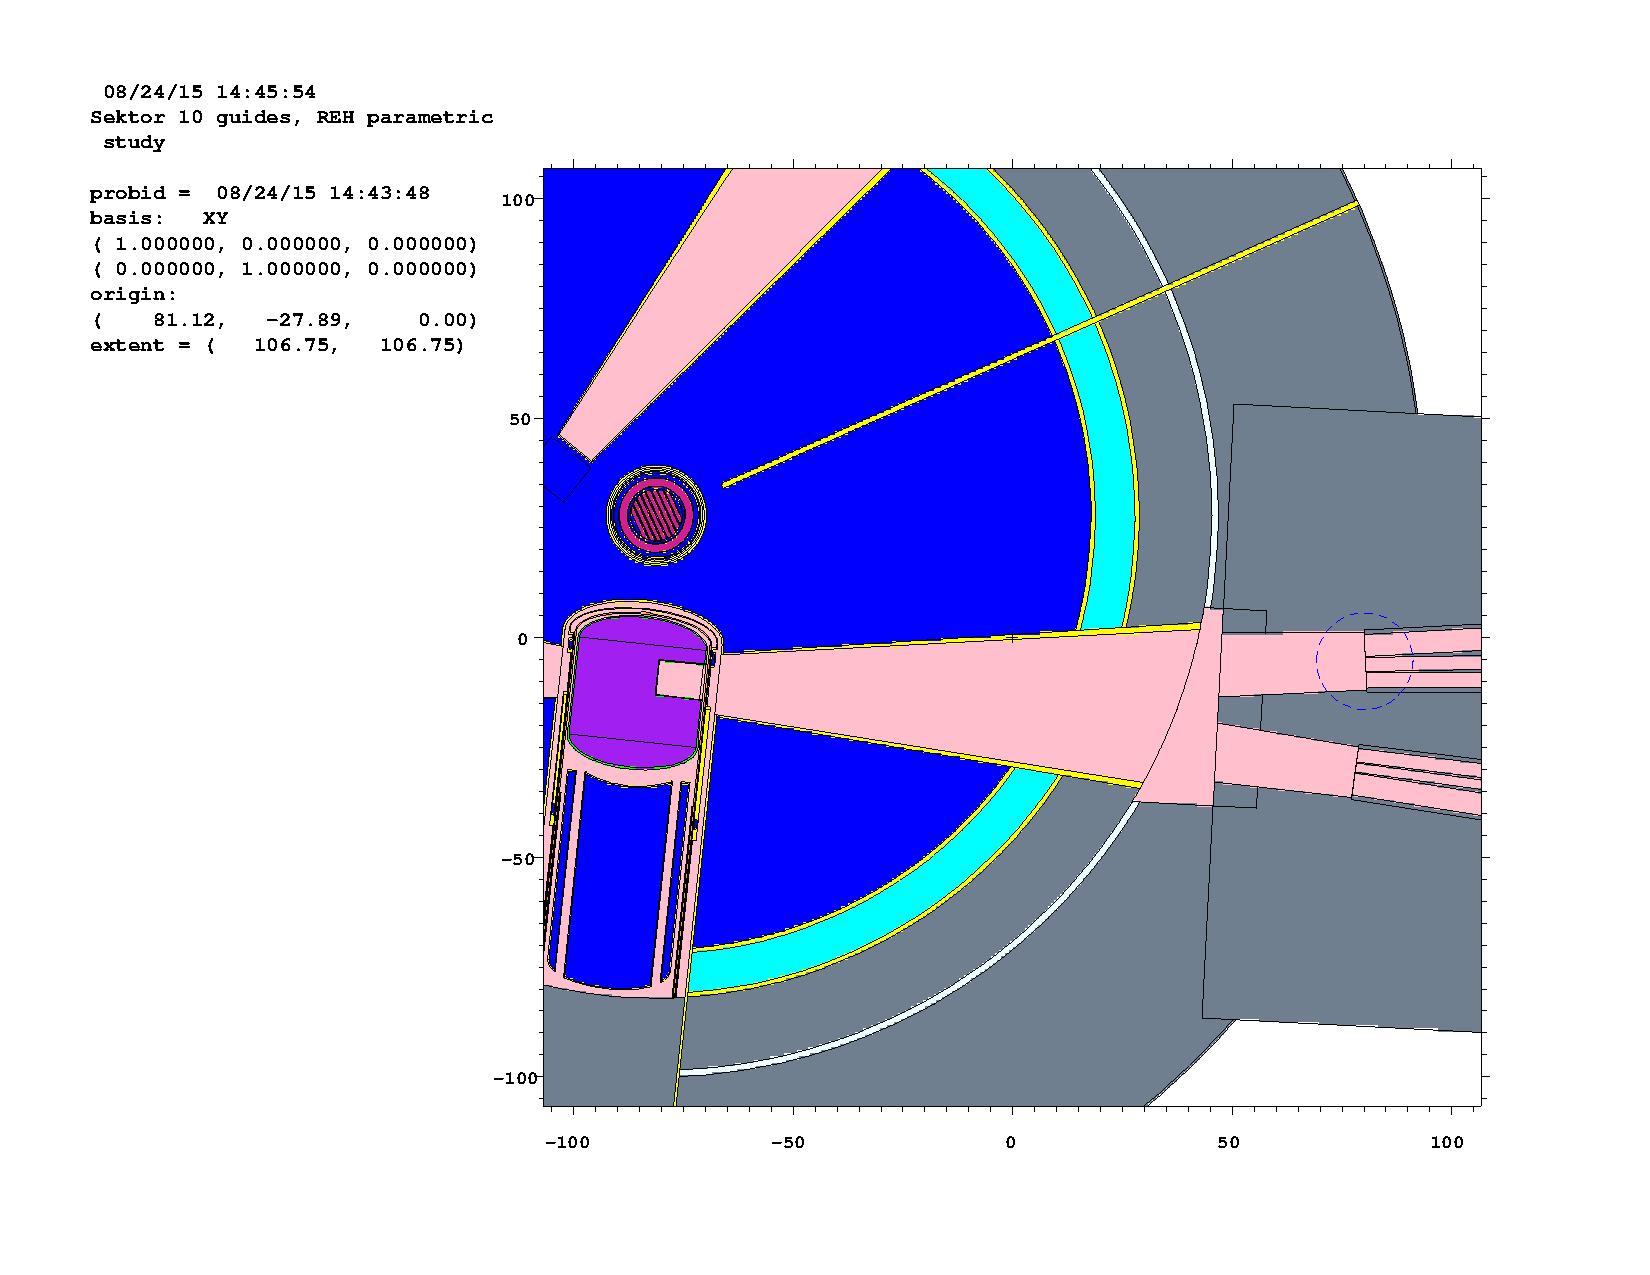
\includegraphics[trim={9.2cm 8cm 4cm 8cm},clip]{graphics/geom.pdf}
\end{center}
\caption{\label{geom}A horizontal slice through the MCNP simulation geometry showing the target (magenta), moderator tank (blue), cold source (purple), nozzle (pink), and neutron guide entrance (grey with circle).}
\end{figure}

\section{Variance Reduction}

Two variance reduciton methods were used in conjunction in order to perform the calculations in a reasonable amount of time.  First, mesh-based weight windows were generated based on the response of a point detector located 75 cm from the neutron guide entrance.  These windows serve to increase the number of neutrons that scatter inside the cold source while preserving the mean particle weight of an analog simulation by casusing the neutrons in the moderator tank to carry a higher weight then be split into many lower-weight particles when they enter the cold source volume.  

The second variance reduction method used is a ``DXTRAN'' sphere.  This tool is a non-physical sphere that is placed around the guide entrance that causes neutrons to be generated on its surface.  Whenever a neutron undergoes a scattering reaction, the probability of scattering into the sphere's direction is calculated, a line is traced from the scattering location to the sphere's surface, and a neutron is generated there with a weight reduced by the scattering probability and the optical thickness of the medium in between.  The generated neutrons are then transported normally inside the sphere \cite{mcnp}.  This method served to preferentially scatter neutrons into the direction of the neutron guide.

\section{Neutron Guide Response} 

In conjunction with the variance reduction methods described in the previous section, an approximation to how the neutron geuides transport neutrons was also used.  A patch was developed at ORNL and PSI that implements the McStas guide reflectivity model in MCNPX 2.5.0 and 2.7.0 \cite{mcnp_reflectivity, EK_reflectivity}, but the model is analog and is not fully compatible with DXTRAN spheres.  The implmentation is analog in the sense that if a neutron is sampled to \emph{not} reflect on a guide surface, it is transmitted into the next cell.  This means that neutron paths have to be sampled multiple times to account for any reflectivity losses, which slows the simulation down.  

Also, some stability issues were encountered while using the reflectivtity patch in conjunction with the DXTRAN sphere.  In order to ensure stable runs, a simulation was done first where a surface source was written at the guide entrance surface where any neutrons entering the guide were recorded and terminated.  This source was used in a second simulation with the guide reflecitvity turned on and used to transport the entering neutrons to the end of the guide where a tally was scored.  Again, this process slowed the simulation down and made studies with many cases more difficult.  An approximaiton to the guide response was used to eliminate the need for a second run to simply get the neutrons to the end of the guide.


\subsection{Guide Reflectivity}

model
guide parameters

\cite{mcnpx_reflectivity}


\subsection{Reconstruction}

method for entry
plot of transfer curves and/or contour plot


\subsection{Self-Consistency Test}

plot of benchmark

\section{REH Parametric Study in the Horizontal Plane}


\subsection{Parameters}

plot of reh and angles
summary of cases


\subsection{Study Results}

plot of spectral band
plot of geometry in XY


\section{Conculsions}

28\% is great



\section{Future Work}

all that jazz



\section{References}

\subsection{Using \BibTeX}
We highly recommend the {\ttfamily\textbf\selectfont iopart-num} \BibTeX\ package by Mark~A~Caprio \cite{iopartnum}, which is included with this documentation.


\begin{figure}[h]
\begin{minipage}{14pc}

\includegraphics[width=14pc]{name.eps}
\caption{\label{label}Figure caption for first of two sided figures.}
\end{minipage}\hspace{2pc}%
\begin{minipage}{14pc}

\includegraphics[width=14pc]{name.eps}
\caption{\label{label}Figure caption for second of two sided figures.}
\end{minipage} 
\end{figure}

\begin{figure}[h]

\includegraphics[width=14pc]{name.eps}\hspace{2pc}%
\begin{minipage}[b]{14pc}\caption{\label{label}Figure caption for a narrow figure where the caption is put at the side of the figure.}
\end{minipage}
\end{figure}


\section*{References}
\begin{thebibliography}{9}
\bibitem{iopartnum} IOP Publishing is to grateful Mark A Caprio, Center for Theoretical Physics, Yale University, for permission to include the {\tt iopart-num} \BibTeX package (version 2.0, December 21, 2006) with  this documentation. Updates and new releases of {\tt iopart-num} can be found on \verb"www.ctan.org" (CTAN). 
\end{thebibliography}

\end{document}


